\documentclass{beamer}
\usetheme{Berlin}

\usepackage{datetime}
\usepackage{amsmath}

\title{Analysis of the Committeeless Proof-of-Stake protocol: searching for a better point of operation}
\author{Vinícius Peixoto\inst{1} \and Marco Aurélio Amaral Henriques\inst{1}}
\institute{\inst{1} Faculdade de Engenharia Elétrica e de Computação (FEEC) - Unicamp}
\date{18 de Setembro de 2023}

\begin{document}
\frame{\titlepage}

\section{Introdução}
\subsection{O que são blockchains?}
\begin{frame}
\begin{itemize}
    \item Livro-razão distribuído, imutável, aberto e descentralizado
    \item Unidade básica de dados: \textbf{bloco}
    \item Blocos são criados em intervalos definidos de tempo: \textbf{rodada}
    \item Blocos são ligados matematicamente entre si
\end{itemize}

\begin{figure}
    \centering
    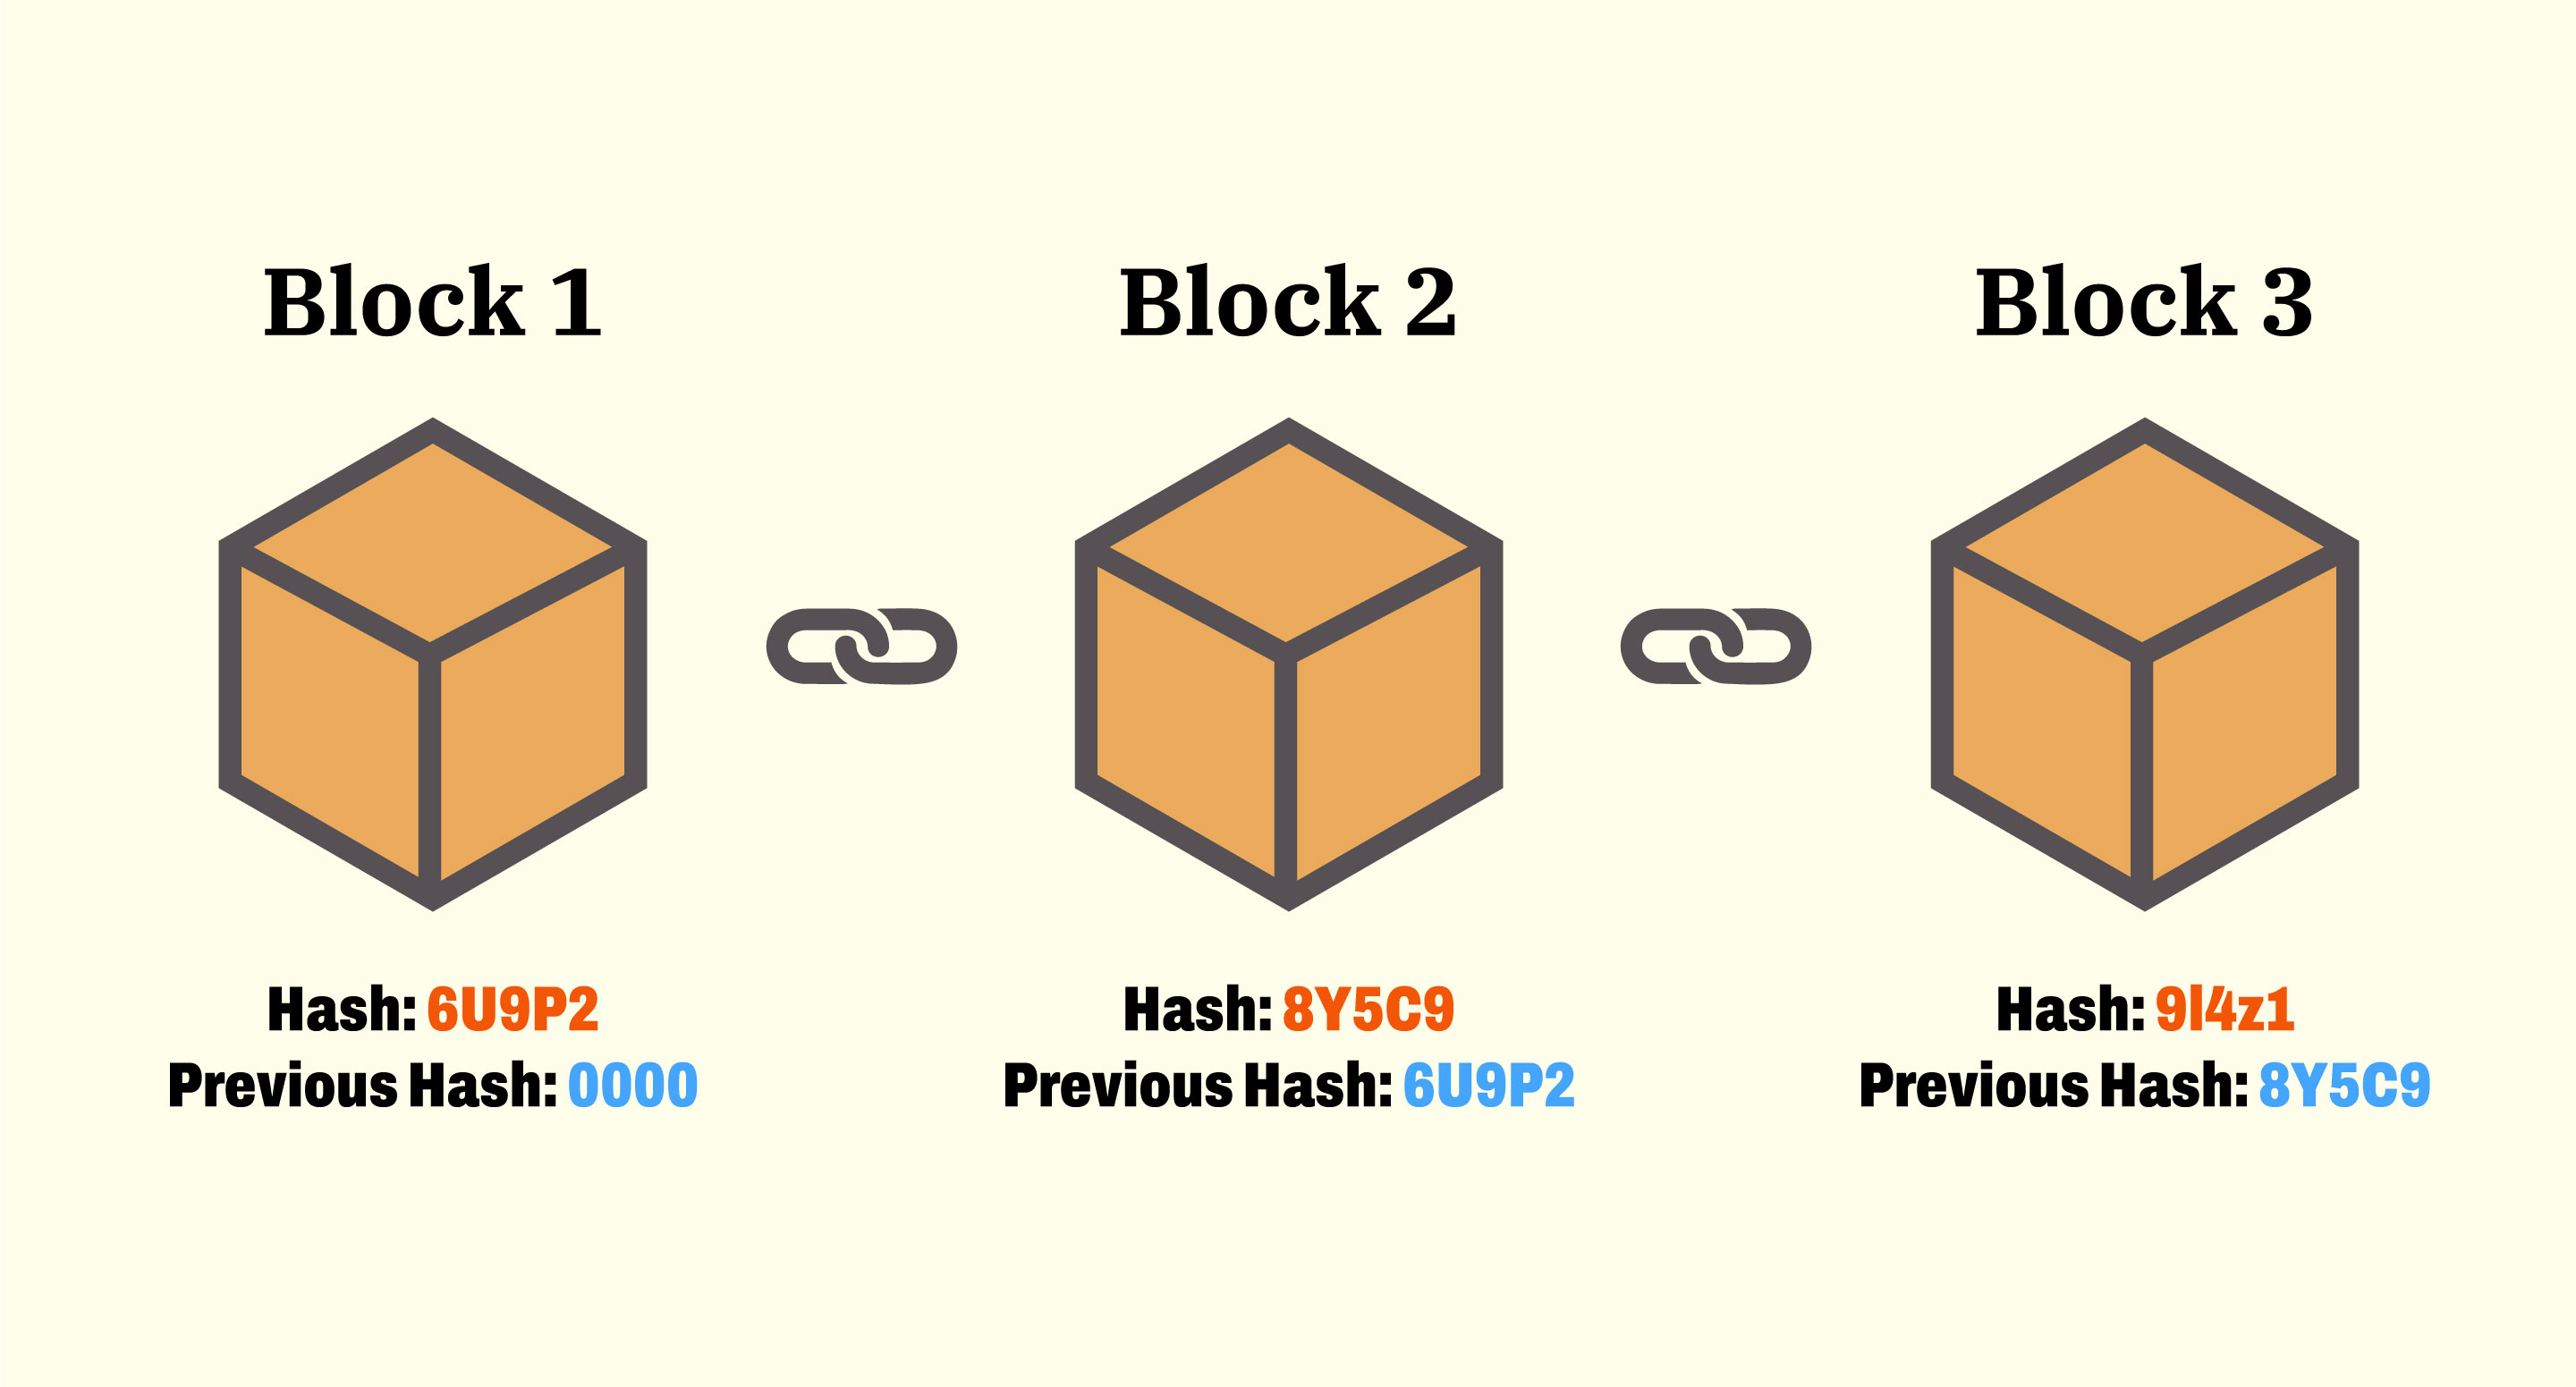
\includegraphics[width=0.6\textwidth]{images/blocks.jpg}
\end{figure}
\end{frame}

\begin{frame}
\begin{itemize}
    \item Blockchains como bancos de dados distribuídos: redes peer-to-peer
    \item Grande quantidade de nós na rede, porém \textbf{apenas um bloco por rodada}
    \item Necessidade de sincronização
    \item \textbf{Mecanismo de consenso distribuído}
\end{itemize}
\end{frame}

\subsection{Mecanismos de consenso}
\begin{frame}
Proof-of-Work (PoW):
\begin{itemize}
    \item Solução de um problema computacionalmente caro
    \item Quem resolver primeiro publica o bloco
    \item Encontrar $n$ tal que $h(n \parallel \text{block}) < 2^d$ ($d$ ajustável)
    \item Grande desperdício de energia: trabalho de todos os nós exceto o sorteado é jogado fora
\end{itemize}
\end{frame}

\begin{frame}
Proof-of-Stake:
\begin{itemize}
    \item Alternativa mais energeticamente eficiente ao PoW
    \item Nós depositam uma quantidade de \textit{stake} para fazerem parte de um \textit{comitê de validação}
    \item Um membro do comitê é sorteado a cada rodada para gerar um bloco
    \item Membros fazem um processo de votação para validar e eleger o bloco
\end{itemize}
\end{frame}

\begin{frame}
\begin{itemize}
    \item Problema: o comitê de validação é uma superfície de ataque
    \item Foram propostos diversos ataques [Neuder 2021, Schwarz-Schilling 2022]
    \begin{itemize}
        \item Estima-se que organizações com menos de 1/3 do stake consigam comprometer o consenso
    \end{itemize}
    \item \textbf{Pergunta}: é possível chegar a um consenso sem um comitê de validação?
\end{itemize}
\end{frame}

\section{O mecanismo CPoS}
\subsection{Visão geral}
\begin{frame}
Committeeless Proof-of-Stake (CPoS): 
\begin{itemize}
    \item Ideia central: \textit{verifiable random functions} $\rightarrow$ sorteios determinísticos
    \item Vários blocos gerados por rodada; critério determinístico de desambiguação
    \item Todos os nós na rede são responsáveis por validar e propagar blocos
    \item Rede tenta convergir para um consenso de forma totalmente distribuída
\end{itemize}
\end{frame}

\subsection{Mecanismo de sorteio}
\begin{frame}
Sorteio determinístico:
\begin{itemize}
    \item Baseado no esquema Algorand [Gilad, 2017]
    \item Em um sorteio aleatório justo, seja $w_i$ o número de fichas (\textit{stake}) de um nó. Seja $p$ a chance de uma dada ficha ser sorteada. Então a chance de exatamente $k$ entre as $w_i$ fichas serem sorteadas é dada pela distribuição binomial:
        \begin{equation*}
            B(w_i, k, p) = \binom{w_i}{k} p^k (1-p)^{w_i - k}
        \end{equation*}
    \item Sorteio: a partir de um conjunto de hashes, é calculado um número $q \in [0.0, 1.0]$. O total de fichas sorteadas é o maior valor $k$ tal que $q > B(w_i, k, p)$.
\end{itemize}
\end{frame}

\begin{frame}
\begin{figure}
    \centering
    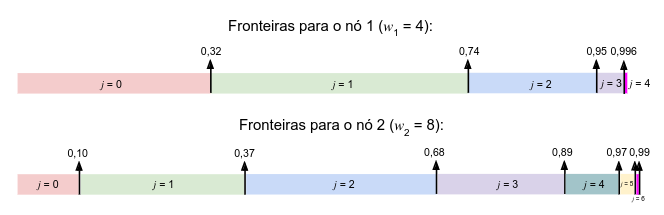
\includegraphics[width=\textwidth]{images/sortition.png}
\end{figure}
\end{frame}

\begin{frame}
\begin{itemize}
    \item Seja $W = \sum w_i$ o \textit{stake} total na rede
    \item É possível provar que o número esperado total de blocos gerados por rodada é dado por $\tau = p \times W$
    \item Desse modo, $p$ é calculado a partir do parâmetro de configuração $\tau$
\end{itemize}
\end{frame}

\subsection{Confirmação de blocos e identificação de forks}
\begin{frame}
Confirmação de blocos:
\begin{itemize}
    \item Baseada nos blocos que chegam até um nó
    \item O nó $i$ calcula, na rodadada $x$, o número total de sorteios bem-sucedidos nos blocos que recebeu: $s_{i}^{x}$
    \item Se os outros peers na rede estão no mesmo fork que $i$, ele espera ver em média $\tau$ sorteios bem sucedidos por rodada
    \item Nó calcula o número de sorteios médio: $ \bar{s} = \frac{1}{\Delta_r} \sum s_i^x$
    \item Bloco confirmado quando $\bar{s}$ se torna suficientemente próximo de $\tau$
\end{itemize}
\end{frame}

\begin{frame}
\begin{itemize}
    \item O processo de confirmação exige que os nós recebam uma quantidade suficientemente grande de blocos
    \item Contudo, o parâmetro $\tau$ controla o número total de blocos gerados
    \item Além disso, um possível ataque: nós não divulgam blocos quando são sorteados
    \item Investigação deste trabalho: \textbf{influência de $\tau$ na performance e resiliência da rede}

\end{itemize}
\end{frame}

\section{Resultados parciais}
\subsection{Metodologia}
\begin{frame}
\begin{itemize}
    \item Experimento 1: influência de $\tau$ em uma rede saudável
    \begin{itemize}
        \item 25 peers no total
        \item Cada peer conhece outros 5 peers
        \item Peers honestos (divulgam blocos)
    \end{itemize}
    \item Experimento 2: influência de $\tau$ em uma rede desonesta
    \begin{itemize}
        \item 30 peers no total
        \item 5 deles ($\approx$ 16\%) não divulgam nós (desonestos)
        \item Topologia de rede conexa
    \end{itemize}
\end{itemize}
\end{frame}

\begin{frame}
\begin{itemize}
    \item Tempo de rodada de 5s
    \item Nós geram blocos vazios (somente headers)
    \item Média de 10 execuções para cada experimento
    \item Infraestrutura de Docker, rodando no Linux 6.4, AMD Ryzen 7 3700X, 32GB RAM
    \item Código disponível em \url{https://github.com/regras/cpos_v2}
\end{itemize}
\end{frame}

\subsection{Resultados}
\begin{frame}
\begin{figure}
    \centering
    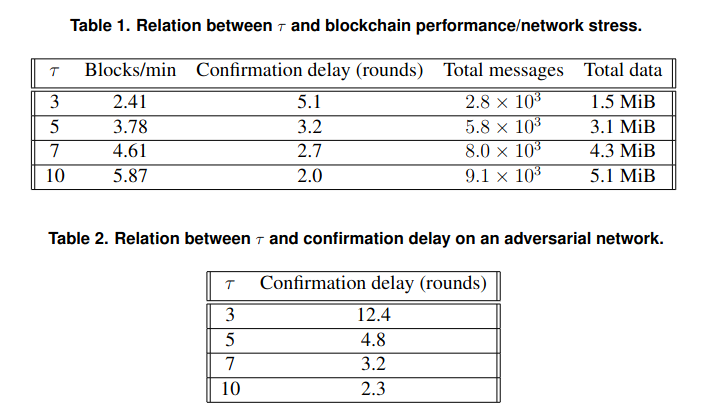
\includegraphics[width=\textwidth]{images/results.png}
\end{figure}
    
\end{frame}

\section{Conclusões e trabalhos futuros}
\subsection{Conclusões}
\begin{frame}
\begin{itemize}
    \item Aumento de $\tau$:
        \begin{itemize}
            \item Maior throughput, menor tempo de confirmação
            \item Aumento da resiliência em presença de nós desonestos
            \item Contudo: umento significativo no número de mensagens e total de dados em circulação
        \end{itemize}
    \item Necessidade de encontrar um equilíbrio entre o valor de $\tau$ e o impacto na rede
        \begin{itemize}
            \item Envio somente de headers até que a rede escolha um bloco; somente então divulgação de blocos ocorre
        \end{itemize}
\end{itemize}
\end{frame}

\begin{frame}
Trabalhos futuros:
\begin{itemize}
    \item Polimentos e melhorias na implementação atual do CPoS
    \item Execução de testes mais extensivos (maior número de blocos, nós distribuídos geograficamente)
    \item Busca de estratégias para minimização do consumo de dados do protocolo
    \item Desenvolvimento de estratégias para punição de nós desonestos
\end{itemize}
\end{frame}

\begin{frame}
    Obrigado!
\end{frame}

\end{document}
